% ---
% id: kempe-chains
% title: Using Kempe chains
% status: in-progress
% parent: five-color
% alternatives: [discharging]
% concepts: [euler-formula, kempe-chain]
% next: Check that Eq. (1) still holds when the vertices are reordered
% created: 2026-09-30
% ---
\section{Five-color theorem: an approach via Kempe chains}

Suppose a coloring $c$ of the planar graph $G-v$ with five colors uses all five colors on the neighbours $v_1,\dots,v_5$ of a degree-five vertex $v$, and
\begin{equation}\label{eq:kempe}
  v_3 \notin \kc{1}{3}{v_1}, \quad c(v_1) \ne c(v_3)
\end{equation}
Then there exists a recolored coloring $c'$ satisfying
\begin{equation}\label{eq:recolor}
  c'(v_1) = c(v_3), \quad c'(v_3) = c(v_3).
\end{equation}

% To check: does \eqref{eq:kempe} still hold when the vertices are reordered?
\begin{figure}[h]
  \centering
  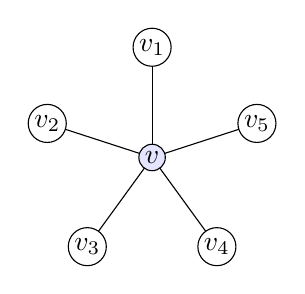
\begin{tikzpicture}
    \foreach \i in {1,...,5} \draw (0,0) -- ({90+72*(\i-1)}:1.4) node[circle,draw,fill=white,inner sep=1pt] {$v_\i$};
    \node[circle,draw,fill=blue!10,inner sep=1pt] at (0,0) {$v$};
  \end{tikzpicture}
  \caption{A degree-five vertex $v$ and its five neighbours $v_1,\dots,v_5$.}
\end{figure}

We have not yet checked whether the $c'$ in \eqref{eq:recolor} can be made to use only four colors.
